\chapter{क्वांटम सांख्यिकी}\label{ch:b3:quantum-statistics}

ताँबे के चालन-इलेक्ट्रॉन हवा से हज़ार गुना सघन एक गैस हैं --- फिर भी
वे ताँबे की ऊष्माधारिता में लगभग कुछ नहीं जोड़ते, और यही कांड पचास
वर्ष तक चिरसम्मत भौतिकी को सताता रहा। रुबिडियम का एक बादल, केल्विन के
अरबवें हिस्सों तक ठंडा किया गया, अचानक दस हज़ार परमाणु गहरी किसी एक
ही क्वांटम अवस्था में ढह जाता है। सूर्य जितने द्रव्यमान और पृथ्वी
जितने आकार का कोई मरा हुआ तारा और सिकुड़ने से इनकार कर देता है, और
उसे अपवर्जन सिद्धांत के सिवा कुछ नहीं थामे रहता। तीनों भौतिकी का एक ही
अध्याय हैं: किसी गैस का क्या होता है जब $n\lambda_T^3 \sim 1$ हो और
\cref{ch:b3:grand-canonical} के अधिभोग-सूत्र बोल्ट्ज़मान से हट जाएँ।
फ़र्मिऑन सागर बनाते हैं --- ठंडे, दृढ़, दबे हुए; और बोसॉन संघनित ---
मिलनसार, संसक्त, अतितरल। फ़र्मी सागर के मौन बहुमत और संघनित की भगदड़
के बीच आधुनिक संघनित-पदार्थ तथा निम्नताप भौतिकी का अधिकांश बसा है,
और तारों की नियति भी।

\section{अधिभोगों की गैसें}

\begin{proposition}[क्वांटम गैस का यंत्र]\label{prop:b3:quantum-statistics:machinery}
\index{अवस्था घनत्व}
किसी बक्से में अन्योन्यक्रियाहीन कणों के लिए स्तरों पर योग
\cref{prop:b3:schrodinger-three-dimensions:counting} के \omterm{prop:b3:schrodinger-three-dimensions:counting}{अवस्था घनत्व}
पर समाकल बन जाते हैं (प्रति चक्रण
अवस्था, $g(\epsilon) = (V/4\pi^2)(2m/\hbar^2)^{3/2}\sqrt\epsilon$):
\[
N = \int_0^\infty g(\epsilon)\,\bar n(\epsilon)\,\dd\epsilon ,
\qquad
E = \int_0^\infty g(\epsilon)\,\bar n(\epsilon)\,\epsilon\,
\dd\epsilon ,
\]
जहाँ $\bar n$ फ़र्मी--डिराक या बोस--आइंस्टाइन अधिभोग है। पहला
समीकरण $\mu(T, n)$ तय करता है; और दूसरा
ऊष्मागतिकी देता है। विरल सीमा $n\lambda_T^3 \ll 1$ में दोनों
सांख्यिकियाँ बोल्ट्ज़मान पर ढह जाती हैं और चिरसम्मत गैस लौट आती है;
क्वांटम प्रांत वहीं शुरू होते हैं जहाँ तरंग-पुंज एक-दूसरे को छू लें।
\end{proposition}
\admitted

\section{फ़र्मी सागर}

\begin{theorem}[अपह्रासित फ़र्मी गैस]\label{thm:b3:quantum-statistics:fermi}
\index{फ़र्मी ऊर्जा}\index{अपह्रासन दाब}
$T = 0$ पर फ़र्मिऑन हर स्तर को \emph{\omterm{thm:b3:quantum-statistics:fermi}{फ़र्मी
ऊर्जा}} तक भर देते हैं
\[
E_{\text{F}} = \frac{\hbar^2}{2m}\,(3\pi^2n)^{2/3}
\qquad (\text{चक्रण } \tfrac12) ,
\]
जहाँ प्रति कण माध्य ऊर्जा $\tfrac35 E_{\text{F}}$ है और
\emph{\omterm{thm:b3:quantum-statistics:fermi}{अपह्रासन दाब}}
\[
P = \frac25\,n\,E_{\text{F}} \;\propto\; n^{5/3} :
\]
अर्थात् परम शून्य पर एक दाब, जिसका उद्गम विशुद्ध क्वांटम है --- हर
धातु की इलेक्ट्रॉन गैस की कड़ाई और मरे हुए तारों का सहारा।
$0 < T \ll T_{\text{F}} = E_{\text{F}}/k_{\text{B}}$ पर
इस \emph{फ़र्मी सागर} की सतह के $\sim k_{\text{B}}T$ भीतर वाले
इलेक्ट्रॉन ही किसी बात पर अनुक्रिया कर सकते हैं: और अंश
$\sim T/T_{\text{F}}$ ही धात्विक व्यवहार की मूल कुंजी है।
\end{theorem}

\begin{proof}[आंशिक उपपत्ति]
$g(\epsilon)$ को $E_{\text{F}}$ तक भरिए: $N = \int_0^{
E_{\text{F}}}g\,\dd\epsilon$ को उलटने पर कथित $E_{\text{F}}$ मिलता है
(\cref{exo:b3:schrodinger-three-dimensions:8}); और एक और समाकल से
$\langle\epsilon
\rangle = \tfrac35 E_{\text{F}}$। दाब: बक्से को दबाने पर हर स्तर
$V^{-2/3}$ की तरह चढ़ता है, अतः $E
\propto V^{-2/3}$ और $P = -\partial E/\partial V = \tfrac23 E/V$
--- और $E = \tfrac35 NE_{\text{F}}$ के साथ, वही कथित नियम।
\end{proof}

\begin{omfigure}
\begin{tikzpicture}
  \begin{axis}[omaxis, axis x line=bottom, axis y line=left,
    width=11.2cm, height=5.2cm, xmin=0, xmax=1.6, ymin=0, ymax=1.2,
    xlabel={$\epsilon/E_{\text{F}}$}, ylabel={अधिभोग $\bar n$},
    xlabel style={at={(axis description cs:0.5,-0.11)}, anchor=north},
    xtick={1}, ytick={0.5,1}, clip=false]
    \addplot[omDef, very thick, domain=0:1.6, samples=250]
      {1/(exp((x-1)/0.05)+1)};
    \addplot[gray, dashed, domain=0:1] {1};
    \fill[omThm!25] (axis cs:0.85,0) -- (axis cs:0.85,0.953)
      .. controls (axis cs:0.95,0.85) .. (axis cs:1.0,0.5)
      .. controls (axis cs:1.05,0.15) .. (axis cs:1.15,0.047)
      -- (axis cs:1.15,0) -- cycle;
    \node[omThm, font=\scriptsize, anchor=west] at (axis cs:1.07,0.72)
      {तापीय कोश, $\sim k_{\text{B}}T$};
    \draw[->, omThm] (axis cs:1.06,0.66) -- (axis cs:1.0,0.47);
    \node[font=\scriptsize, anchor=west] at (axis cs:0.07,0.35)
      {गहरी अवस्थाएँ जमी हुईं};
  \end{axis}
\end{tikzpicture}

{\small $T \ll T_{\text{F}}$ पर फ़र्मी सागर: अधिभोग एक
ज़रा-सी धुँधली सीढ़ी है। गहरे इलेक्ट्रॉन न प्रकीर्ण हो सकते हैं, न
अवशोषित कर सकते हैं, न अनुक्रिया कर सकते हैं --- हर सुलभ अवस्था भरी
है; और धात्विक भौतिकी का सारा कारोबार सतह के उस पतले तापीय कोश में
होता है।}
\end{omfigure}

\begin{example}[ऊष्माधारिता का कांड, सुलझा]\label{ex:b3:quantum-statistics:heat}
\index{इलेक्ट्रॉनी ऊष्माधारिता}
चिरसम्मत ढंग से ताँबे के प्रति परमाणु एक मुक्त इलेक्ट्रॉन को
ऊष्माधारिता में $\tfrac32
k_{\text{B}}$ जोड़ना चाहिए --- अर्थात् द्यूलों--प्टी के ऊपर $50\%$।
मापा गया: कमरे के ताप पर लगभग $1\%$। सागर इसे
समझा देता है: $T_{\text{F}} \approx \qty{8e4}{K}$ के साथ केवल
$\sim T/T_{\text{F}} \approx 0.4\%$ अंश के इलेक्ट्रॉन ही
तापीय रूप से उत्तेजित हो सकते हैं, हर एक $\sim k_{\text{B}}T$ जितना:
\[
C_{\text{el}} \approx \frac{\pi^2}{2}\,
Nk_{\text{B}}\,\frac{T}{T_{\text{F}}}
\]
(यही यथार्थ ज़ोमरफ़ेल्ट गुणांक है;
\cref{exo:b3:quantum-statistics:12})। $T$ में रैखिक होने के कारण वह
साधारण तापों पर जालक के $T^3$ के नीचे दब जाता है, पर कुछ ही केल्विन
से नीचे \emph{हावी} हो जाता है --- ठीक जैसा कैलोरीमापी पाते हैं, और
इस तरह एक ही झटके में उन इलेक्ट्रॉनों की पहेली सुलझ जाती है जो धारा
ढोते हैं पर ऊष्माधारिता नहीं।
\end{example}

\begin{example}[अपवर्जन से थमे तारे]\label{ex:b3:quantum-statistics:dwarf}
\index{श्वेत वामन}
कोई \omterm{ex:b3:quantum-statistics:dwarf}{श्वेत वामन} (\cref{exo:b3:identical-particles:11}) गुरुत्व को
इलेक्ट्रॉनों के \omterm{thm:b3:quantum-statistics:fermi}{अपह्रासन दाब} से संतुलित करता है। चूँकि तारे के
सिकुड़ने पर $P \propto
n^{5/3}$ गुरुत्व की माँगों से तेज़ी से कड़ा होता है, इसलिए किसी भी
मामूली द्रव्यमान पर एक संतुलन-त्रिज्या मिल जाती है --- और वह भी
अजीब मापन $R \propto M^{-1/3}$ के साथ: \emph{भारी वामन अधिक छोटे
होते हैं}। और अधिक दबाने पर इलेक्ट्रॉन आपेक्षिकीय हो जाते हैं,
दाब-नियम नरम पड़कर $n^{4/3}$ हो जाता है, और संतुलन किसी एक ही
द्रव्यमान पर टूट जाता है --- चंद्रशेखर सीमा $M_{\text{Ch}} \approx
1.4\,M_\odot$ (\cref{pb:b3:quantum-statistics:1}) --- उसके आगे
न्यूट्रॉन तारे तक ढहना: नाभिकीय घनत्व पर न्यूट्रॉनों का एक फ़र्मी
सागर, वही भौतिकी $10^{14}$ गुने घनत्व पर।
\end{example}

\section{बोसॉनों की भगदड़}

\begin{theorem}[बोस--आइंस्टाइन संघनन]\label{thm:b3:quantum-statistics:bec}
\index{बोस--आइंस्टाइन संघनन}
$N$ संरक्षित बोसॉनों की किसी गैस के लिए उत्तेजित अवस्थाएँ अधिक से
अधिक $N_{\max}(T) = 2.612\,V/\lambda_T^3$ कण रख सकती हैं
($g\bar n_{\text{BE}}$ का समाकल, उसकी छत $\mu \to 0$ पर)। क्रांतिक
ताप से नीचे
\[
k_{\text{B}}T_{\text{c}} = \frac{2\pi\hbar^2}{m}
\Big(\frac{n}{2.612}\Big)^{2/3}
\quad\text{(तुल्यतः } n\lambda_{T_{\text{c}}}^3 = 2.612
\text{)} ,
\]
अतिरेक के पास एकमात्र मूल अवस्था के सिवा जाने की कोई जगह नहीं बचती:
एक \emph{स्थूल} जनसंख्या
\[
\frac{N_0}{N} = 1 - \Big(\frac{T}{T_{\text{c}}}\Big)^{3/2}
\]
एक ही क्वांटम अवस्था में संघनित हो जाती है --- पदार्थ किसी विशाल
तरंग फलन की तरह बरतता हुआ। आइंस्टाइन ने 1925 में बोस की फ़ोटॉन
सांख्यिकी से इसकी भविष्यवाणी की; और 1995 में विरल रुबिडियम में
$T_{\text{c}} \approx \qty{100}{nK}$ पर यह साकार हुआ (नोबेल 2001),
जिसकी घोषणा उस चुगली करते \emph{द्विशिखरी} वेग-वितरण ने की: एक तापीय
बादल, जिसके बीच से शून्य-वेग वाले संघनित की सुई उठती हुई।
\end{theorem}
\admitted

\begin{omfigure}
\begin{tikzpicture}
  \begin{axis}[omaxis, axis x line=bottom, axis y line=left,
    width=6.6cm, height=5.0cm, xmin=0, xmax=1.35, ymin=0, ymax=1.1,
    xlabel={$T/T_{\text{c}}$}, ylabel={$N_0/N$},
    xlabel style={at={(axis description cs:0.5,-0.12)}, anchor=north},
    xtick={0.5,1}, ytick={0.5,1}, clip=false]
    \addplot[omDef, very thick, domain=0:1, samples=100]
      {1-x^1.5};
    \addplot[omDef, very thick, domain=1:1.35] {0};
    \node[omDef, font=\scriptsize, anchor=west] at (axis cs:0.1,0.25)
      {संघनित अंश};
  \end{axis}
  \begin{axis}[omaxis, axis x line=bottom, axis y line=left,
    width=6.6cm, height=5.0cm, xmin=-3, xmax=3, ymin=0, ymax=1.35,
    xshift=7.2cm,
    xlabel={वेग}, ylabel={परमाणु-गिनती},
    xlabel style={at={(axis description cs:0.5,-0.12)}, anchor=north},
    xtick=\empty, ytick=\empty, clip=false]
    \addplot[omExo, thick, domain=-3:3, samples=120]
      {0.42*exp(-x*x/1.8)};
    \addplot[omThm, very thick, domain=-3:3, samples=200]
      {0.42*exp(-x*x/1.8)+0.85*exp(-x*x/0.045)};
    \node[omExo, font=\scriptsize, anchor=west] at (axis cs:1.15,0.5)
      {तापीय बादल};
    \node[omThm, font=\scriptsize, anchor=west] at (axis cs:0.3,1.2)
      {संघनित की सुई};
  \end{axis}
\end{tikzpicture}

{\small बाएँ: $T_{\text{c}}$ से नीचे मूल अवस्था की जनसंख्या
स्थूल हो जाती है। दाएँ: 1995 का चिह्न --- छोड़कर चित्रित करने पर
बादल एक चौड़ा तापीय वितरण दिखाता है, जिसमें एक सँकरी
शून्य-वेग शलाका है: एक ही क्वांटम अवस्था, कैमरे को दिखती हुई।}
\end{omfigure}

\begin{example}[हीलियम, अनुभवी अतितरल]\label{ex:b3:quantum-statistics:helium}
\index{अतितरलता}
द्रव $^4$He (बोसॉनी) $T_\lambda = \qty{2.17}{K}$ पर एक
\emph{अतितरल} में बदल जाता है: महीन से महीन केशिकाओं से होकर शून्य
श्यानता, पात्र की दीवारों पर फ़िल्म-बहाव, फ़व्वारा-प्रभाव, और
$h/m$ की इकाइयों में क्वांटित परिसंचरण --- अर्थात् किसी संघनित की
स्थूल कला काम पर, जो अन्योन्यक्रियाओं के कारण आदर्श-गैस भविष्यवाणी
(हीलियम के घनत्व के लिए $\qty{3.1}{K}$) से खिसकी हुई है, पर स्पष्ट
रूप से वही परिघटना है। फ़र्मिऑनी $^3$He अकेले संघनित नहीं हो सकता:
उसके परमाणुओं को पहले \emph{युग्म} बनाने पड़ते हैं (किसी
अतिचालक के इलेक्ट्रॉनों की तरह, \cref{ch:b3:electrons-in-solids}),
जिससे वे संयुक्त बोसॉन बनें --- और अतितरलता आ भी जाती है, पर
\qty{2.6}{mK} पर, हज़ार गुना ठंडे: दो समस्थानिक, एक सीख ---
सांख्यिकी ही नियति है।
\end{example}

\begin{method}[कौन-सी सांख्यिकी, कौन-सा प्रांत]\label{met:b3:quantum-statistics:method}
(1) पहले $n\lambda_T^3$ निकालिए: $\ll1$ का अर्थ है बोल्ट्ज़मान, और
\omterm{thm:b3:canonical-ensemble:boltzmann}{विहित समुदाय} ही काफ़ी है। (2) अपह्रासित फ़र्मिऑन:
$E_{\text{F}}$ और $T/T_{\text{F}}$ में सोचिए; अनुक्रियाएँ
(ऊष्माधारिता, प्रवृत्ति, प्रकीर्णन) या तो $T/T_{\text{F}}$ गुणक ढोती
हैं या केवल फ़र्मी सतह का नमूना लेती हैं। (3) अपह्रासित बोसॉन: $T$
की $T_{\text{c}}$ से तुलना कीजिए; उससे नीचे गैस को संघनित और तापीय
बादल में बाँट दीजिए। (4) दाब: $n^{5/3}$ की फ़र्मिऑनी कड़ाई (या
$n^{4/3}$ आपेक्षिकीय) उस चीज़ के सामने जो दबा रही हो। (5) संयुक्त
कण: सांख्यिकी चुनने के लिए घटक फ़र्मिऑन गिनिए --- और याद रखिए कि
युग्मन एक सांख्यिकी को दूसरी में बदल सकता है।
\end{method}

\begin{omfigure}
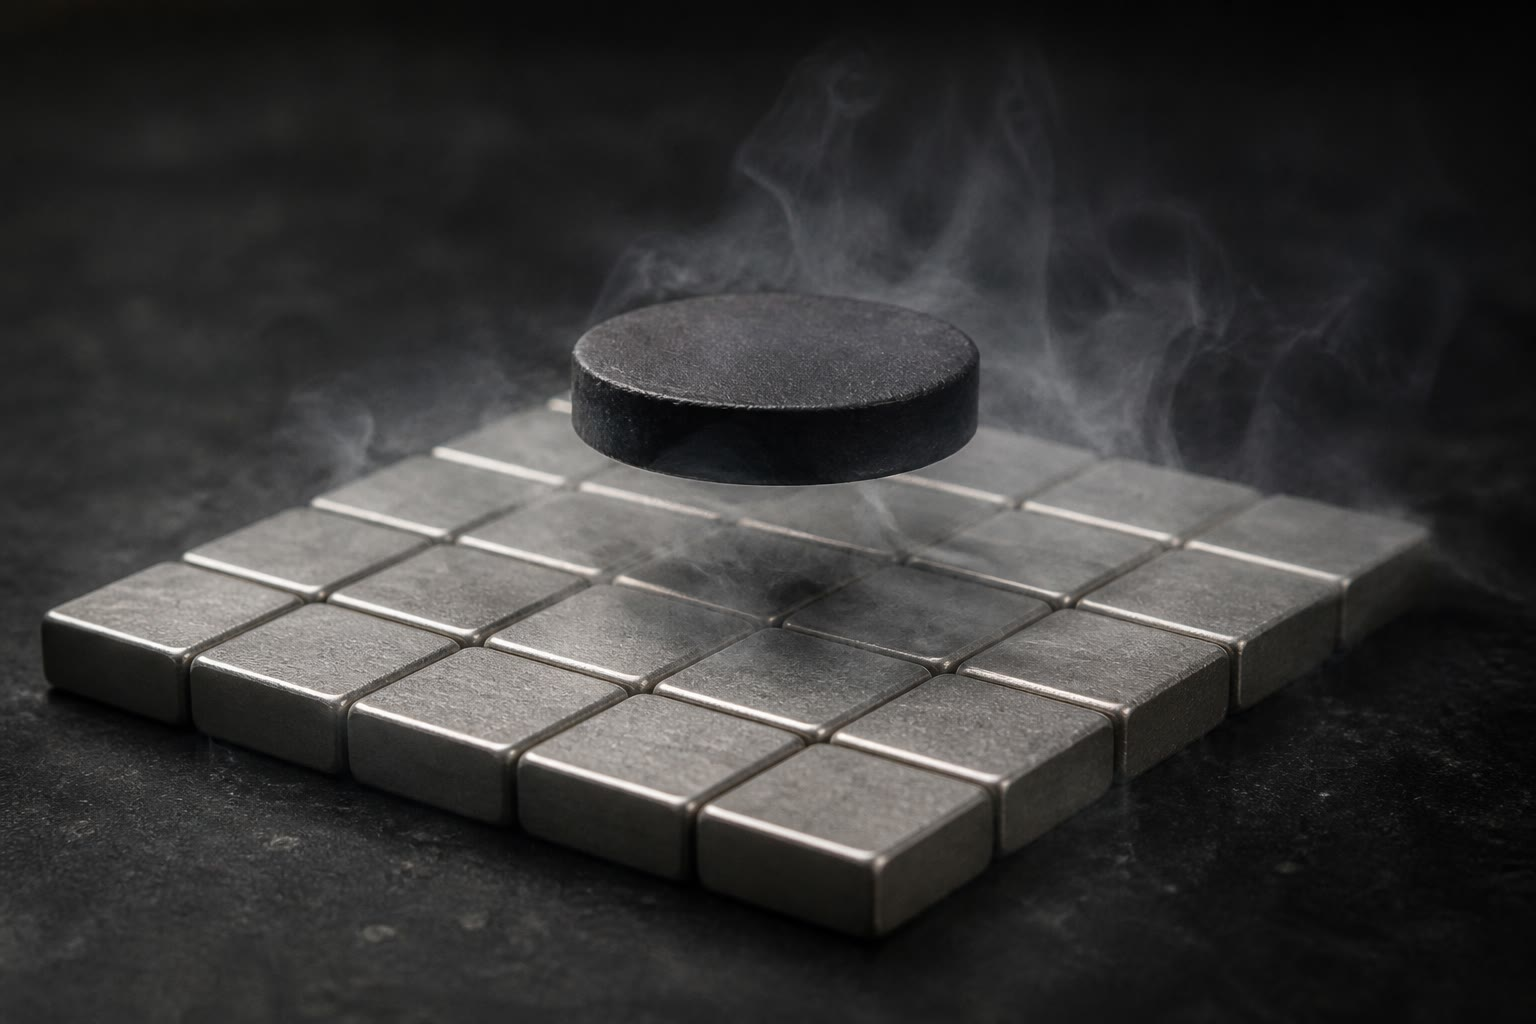
\includegraphics[width=0.58\linewidth]{images/book5/ai/b5-25-superconductor-levitation.jpg}

{\small कोई अतिचालक किसी चुंबक की क्षेत्र-रेखाओं को परे धकेलकर उसे हवा में थामे हुए: अपने क्रांतिक ताप से नीचे इलेक्ट्रॉन-तरल एक ही स्थूल क्वांटम अवस्था में संघनित हो जाता है --- अपह्रासन की भौतिकी, जो एक चकती को हवा में टिकाए रखती है।}
\end{omfigure}

\section{अभ्यास}

\begin{exercise}[$\star$]\label{exo:b3:quantum-statistics:1}
$E_{\text{F}}$ और $T_{\text{F}}$ निकालिए: (क) ताँबे के लिए
($n = \qty{8.5e28}{m^{-3}}$); (ख) सोडियम के लिए
($\qty{2.5e28}{m^{-3}}$); (ग) द्रव $^3$He के लिए ($\qty{1.6e28}{m^{-3}}$,
$m = 3u$); (घ) इन्हें कमरे के ताप के सामने क्रम में रखिए और बताइए
कि कौन कब अपह्रासित है।
\end{exercise}

\begin{exercise}[$\star$]\label{exo:b3:quantum-statistics:2}
(क) दिखाइए कि $\langle\epsilon\rangle = \tfrac35 E_{\text{F}}$, $T =
0$ पर। (ख) ताँबे
में इलेक्ट्रॉनों की वर्ग-माध्य-मूल चाल निकालिए। (ग) वह
चाल चिरसम्मत ढंग से किस ताप के तुल्य है? (घ) कोई ठंडी धातु प्रकाश
की गति के सौवें हिस्से पर चलते इलेक्ट्रॉन अपने भीतर रखती है और फिर
भी वह ऊर्जा विकिरित क्यों नहीं कर देती?
\end{exercise}

\begin{exercise}[$\star$]\label{exo:b3:quantum-statistics:3}
ताँबे के इलेक्ट्रॉनों का \omterm{thm:b3:quantum-statistics:fermi}{अपह्रासन दाब}: (क) $P =
\tfrac25 nE_{\text{F}}$ का मान पास्कल और वायुमंडल में निकालिए। (ख)
वह धातु फट क्यों नहीं जाती (कौन पीछे खींचता है)? (ग) यह दाब
संपीडन का विरोध करता है: धातुओं की कम संपीड्यता से जोड़िए। (घ)
आयतन गुणांक $K \sim \tfrac53 P$ आकलिए और ताँबे के मापे गए
\qty{140}{GPa} से तुलिए।
\end{exercise}

\begin{exercise}[$\star$]\label{exo:b3:quantum-statistics:4}
BEC की देहलियाँ। (क) $T_{\text{c}}$ निकालिए, रुबिडियम-87 ($m =
\qty{1.44e-25}{kg}$) के लिए, $n = \qty{e20}{m^{-3}}$ पर। (ख) उसी
$n$ के लिए हाइड्रोजन परमाणुओं का $T_{\text{c}}$ क्या होता? (ग) प्रयोग
मिलिकेल्विन पर सघन गैसों के बजाय नैनोकेल्विन पर विरल गैसें क्यों
काम में लेते हैं (ऊँचे घनत्व और कम ताप पर रासायनिक रूप से क्या होता
है)? (घ) अपनी रुबिडियम संख्याओं पर संगति-नियम $n\lambda_{T_c}^3
= 2.612$ जाँचिए।
\end{exercise}

\begin{exercise}[$\star\star$]\label{exo:b3:quantum-statistics:5}
दो ऊष्माधारिताएँ। किसी धातु में $C = \gamma T +
\beta T^3$ (इलेक्ट्रॉन; जालक)। (क)
\cref{ex:b3:quantum-statistics:heat} और डिबाई-सरीखे जालक-पद
$\beta T^3 = 234\,Nk_{\text{B}}(T/\theta_{\text{D}})^3$ से
ताँबे के लिए संक्रमण-ताप आकलिए
($\theta_{\text{D}} = \qty{343}{K}$, $T_{\text{F}} =
\qty{8.2e4}{K}$)। (ख) \qty{300}{K} पर इलेक्ट्रॉनों का हिस्सा
प्रतिशत में। (ग) \qty{0.1}{K} पर? (घ) प्रयोगकर्ता $C/T$ को
$T^2$ के सामने क्यों आलेखित करते हैं, और उस सरल रेखा का अंतःखंड तथा
ढाल क्या देते हैं?
\end{exercise}

\begin{exercise}[$\star\star$]\label{exo:b3:quantum-statistics:6}
एक सौर द्रव्यमान ($M = \qty{2e30}{kg}$) और पृथ्वी की त्रिज्या
($R = \qty{6.4e6}{m}$) वाला कोई \omterm{ex:b3:quantum-statistics:dwarf}{श्वेत वामन}, प्रति दो न्यूक्लिऑन एक
इलेक्ट्रॉन। (क)
$n_{\text{e}}$ और $E_{\text{F}}$ निकालिए (अनापेक्षिकीय
सूत्र)। (ख) $E_{\text{F}}$ की तुलना $m_{\text{e}}c^2$ से और
भीतरी \qty{e7}{K} पर $k_{\text{B}}T$ से कीजिए: ``ठंडा'' और
``लगभग आपेक्षिकीय'' दोनों को एक साथ उचित ठहराइए। (ग)
\omterm{thm:b3:quantum-statistics:fermi}{अपह्रासन दाब} $\tfrac25 nE_{\text{F}}$ की तुलना
गुरुत्वीय दाब के आकलन $\sim GM^2/R^4$ से कीजिए: क्या वही कोटि? (घ) $M$ बढ़ने पर संतुलन के हर पक्ष
का गुणात्मक रूप से क्या होता है?
\end{exercise}

\begin{exercise}[$\star\star$]\label{exo:b3:quantum-statistics:7}
न्यूट्रॉन पदार्थ। कोई न्यूट्रॉन तारा $M = 1.4\,M_\odot$ को $R
\approx \qty{11}{km}$ में ठूँसता है। (क) न्यूट्रॉन घनत्व निकालिए और
नाभिकीय घनत्व ($\qty{2.3e17}{kg/m^3}$) से तुलिए। (ख) न्यूट्रॉनों के
लिए $E_{\text{F}}$ निकालिए (अनापेक्षिकीय; $m_{\text{n}}c^2
= \qty{939}{MeV}$) और जाँचिए कि वे कितने आपेक्षिकीय हैं। (ग) तारे
के इलेक्ट्रॉन क्यों लुप्त हो गए (प्रतिलोम बीटा क्षय:
$\text{e} + \text{p} \to \text{n} + \nu$ --- किस चीज़ ने
इलेक्ट्रॉनों की $E_{\text{F}}$ से उसकी कीमत चुकवाई)? (घ) इस
पदार्थ की एक चम्मच का भार कितना होगा?
\end{exercise}

\begin{exercise}[$\star\star$]\label{exo:b3:quantum-statistics:8}
बिना संख्या वाले बोसॉन। (क) फ़ोटॉनों का $\mu = 0$ सदा रहता है: वे
\cref{thm:b3:quantum-statistics:bec} वाला संघनन क्यों नहीं कर सकते
(ठंडा करने पर गैस इसके बदले क्या करती है)? (ख) रुबिडियम परमाणुओं के
पास कौन-सा संरक्षण-नियम है जो फ़ोटॉनों के पास नहीं? (ग) 2010 में
किसी रंजक-भरी गुहा में फ़ोटॉन BEC बना \emph{ही} लिया गया, जहाँ
फ़ोटॉन तापीय संतुलन में आते हैं और उनकी संख्या व्यवहारतः नियत रहती
है: उस रंजक-गुहा ने कौन-सी सामग्री लौटा दी?
(घ) किसी क्रिस्टल में फ़ोनॉन: संघनन या नहीं, और क्यों?
\end{exercise}

\begin{exercise}[$\star\star$]\label{exo:b3:quantum-statistics:9}
हीलियम के दो समस्थानिक। (क) आदर्श-गैस वाला $T_{\text{c}}$ निकालिए,
द्रव $^4$He ($n = \qty{2.2e28}{m^{-3}}$, $m = 4u$) के लिए,
और $T_\lambda = \qty{2.17}{K}$ से तुलिए। (ख) सहमति केवल
मोटी-मोटी क्यों है (किसी द्रव में ``आदर्श'' क्या अनदेखा करता है)?
(ग) लगभग उसी घनत्व वाला $^3$He मिलिकेल्विन तक सामान्य बना रहता है:
वह रुकावट और प्रकृति का खोजा हुआ उपाय बताइए। (घ) संयुक्त कणों का
तर्क जाँचिए: किसी $^3$He \emph{युग्म} में सम संख्या में फ़र्मिऑन
होते हैं --- अर्थात् बोसॉन; और $^6$Li में $3\text{p} + 3\text{n}
+ 3\text{e} = 9$ फ़र्मिऑन हैं: उसे वर्गीकृत कीजिए, और उन प्रसिद्ध
शीत-गैस प्रयोगों के नाम लीजिए जो ठीक इसी लीथियम--लीथियम विरोध का
दोहन करते हैं।
\end{exercise}

\begin{exercise}[$\star\star\star$]\label{exo:b3:quantum-statistics:10}
$T_{\text{c}}$, ईमानदारी से। (क) $N_{\text{उत्त}} = \int_0^\infty
g(\epsilon)\dd\epsilon/(\eu^{\beta\epsilon} - 1)$ को $\mu = 0$ पर लिखिए और
$x = \beta\epsilon$ के साथ उसे $N_{\text{उत्त}} =
(V/\lambda_T^3)\cdot\frac{2}{\sqrt\pi}\int_0^\infty\frac{\sqrt
x\,\dd x}{\eu^x - 1}$ तक घटाइए। (ख) $\int_0^\infty\sqrt x\,\dd x/(
\eu^x - 1) = 2.612\,\sqrt\pi/2$ दिया हो, तो वह छत और
$T_{\text{c}}$ पाइए। (ग) संघनित अंश $1 -
(T/T_{\text{c}})^{3/2}$ व्युत्पन्न कीजिए। (घ) वही तर्क किसी
द्विविमीय बक्से में \emph{कोई} संघनन क्यों नहीं देता ($g(
\epsilon)$ कैसे बदलता है, और समाकल के अभिसरण का क्या होता
है)?
\end{exercise}

\begin{exercise}[$\star\star\star$]\label{exo:b3:quantum-statistics:11}
धातुएँ आपस में क्यों जुड़ी रहती हैं। किसी धातु का प्रतिरूप घनत्व
$n$ के इलेक्ट्रॉनों से बनाइए (प्रति इलेक्ट्रॉन \omterm{thm:b3:quantum-statistics:fermi}{फ़र्मी ऊर्जा} की लागत
$\propto n^{2/3}$), जो किसी उदासीनकारी आयन-पृष्ठभूमि से आकर्षित हों
(प्रति इलेक्ट्रॉन कूलॉम लाभ
$\sim -e^2n^{1/3}/4\pi\varepsilon_0$)। (क) प्रति इलेक्ट्रॉन ऊर्जा
$\epsilon(n) = An^{2/3} - Bn^{1/3}$ लिखिए और दिखाइए कि उसका कोई
न्यूनतम है। (ख) दिखाइए कि संतुलन पर इलेक्ट्रॉनों का अंतराल
$a_0$ की कोटि का है --- धात्विक घनत्व संयोग नहीं हैं। (ग) न्यूनतम
पर संसंजन ऊर्जा का पैमाना eV में आकलिए। (घ) इस बद्ध अवस्था में
\omterm{thm:b3:quantum-statistics:fermi}{अपह्रासन दाब} की क्या भूमिका है (कूलॉम पतन को कौन रोकता है)?
\end{exercise}

\begin{exercise}[$\star\star\star$]\label{exo:b3:quantum-statistics:12}
ज़ोमरफ़ेल्ट का कोश, संख्याओं में। (क) तर्क दीजिए: $N$ इलेक्ट्रॉनों
में से केवल $\sim g(E_{\text{F}})k_{\text{B}}T$ सक्रिय कोश में
बैठते हैं, हर एक $\sim k_{\text{B}}T$ अतिरिक्त ऊर्जा लिए: इससे किसी
नियतांक तक $C_{\text{el}}
\sim g(E_{\text{F}})k_{\text{B}}^2T$ व्युत्पन्न कीजिए। (ख)
$g(E_{\text{F}}) = 3N/2E_{\text{F}}$ के साथ $C_{\text{el}} \sim
Nk_{\text{B}}T/T_{\text{F}}$ पुनः पाइए (यथार्थ नियतांक $\pi^2/2$
है)। (ग) वही कोश-तर्क पाउली की ताप-निरपेक्ष चक्रण-प्रवृत्ति देता
है: केवल कोश के इलेक्ट्रॉन ही पलट सकते हैं --- पर कोश $T$ की तरह
बढ़ता है जबकि हर योगदान $1/T$ की तरह गिरता है: वह कटाव दिखाइए। (घ)
अपह्रासित फ़र्मिऑनों के लिए व्यापक सार बताइए: \emph{हर} अनुक्रिया
चिरसम्मत अनुक्रिया गुणा $\sim T/T_{\text{F}}$ है, या उसका
केवल-सतह वाला समरूप।
\end{exercise}

\begin{omfigure}
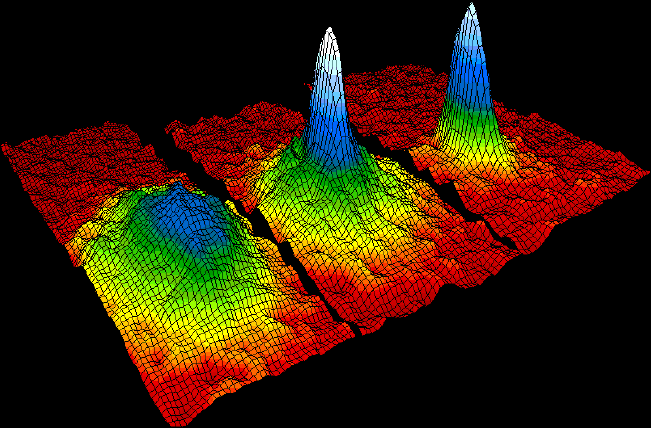
\includegraphics[width=0.55\linewidth]{images/book5/photo-bec-nist.png}

{\small पहला बोस--आइंस्टाइन संघनित (NIST/JILA, 1995, सार्वजनिक डोमेन): बाएँ से दाएँ गैस के ठंडा होते जाने पर रुबिडियम परमाणुओं के वेग-वितरण --- तापीय पहाड़ी ढहकर संघनित की शलाका बन जाती है, भविष्यवाणी के सत्तर वर्ष बाद।}
\end{omfigure}

\section{समस्या: सबसे भारी संभव श्वेत वामन}

\begin{problem}[{सप्ताहांत समस्या --- चंद्रशेखर सीमा, और उसके जलाए
हुए दीपक}]\label{pb:b3:quantum-statistics:1}
1930 में, उन्नीस वर्ष की आयु में, सुब्रह्मण्यन चंद्रशेखर ने
इंग्लैंड जाते जहाज़ पर यह गणना की कि इलेक्ट्रॉनों का अपह्रासन किसी
मरे हुए तारे को केवल किसी निश्चित द्रव्यमान तक ही थाम सकता है। वह
परिणाम --- जिसका एडिंगटन ने कड़वाहट से विरोध किया --- न्यूट्रॉन
तारों, कृष्ण विवरों और उन अधिनवतारा ``मानक दीपकों'' के नीचे बैठा है
जिन्होंने त्वरित होते ब्रह्मांड को उजागर किया। यह समस्या उसे मापन से
गढ़ती है। आँकड़े: $M_\odot =
\qty{2e30}{kg}$; प्रति $\mu_e = 2$ न्यूक्लिऑन एक इलेक्ट्रॉन; $m_{\text{
n}} = \qty{1.67e-27}{kg}$; $\hbar c = \qty{3.16e-26}{J.m}$; $G =
\qty{6.67e-11}{N.m^2/kg^2}$।

\medskip\noindent\textbf{भाग I --- दो ऊर्जाओं का संतुलन।}
द्रव्यमान $M$ और त्रिज्या $R$ वाले किसी तारे के लिए, प्रति एकांक
द्रव्यमान ऊर्जाओं को मापन से बरतिए।
\begin{enumerate}
  \item गुरुत्वीय ऊर्जा: $E_{\text{g}} \sim -GM^2/R$ ---
        उसका उद्गम याद कीजिए।
  \item इलेक्ट्रॉन-गिनती $N_{\text{e}} = M/\mu_e m_{\text{n}}$ और
        घनत्व $n \sim N_{\text{e}}/R^3$: अनापेक्षिकीय \omterm{thm:b3:quantum-statistics:fermi}{फ़र्मी ऊर्जा}
        का पैमाना $M$
        और $R$ के फलन के रूप में लिखिए।
  \item दिखाइए कि कुल गतिज (अपह्रासन) ऊर्जा
        $E_{\text{k}} \sim \hbar^2N_{\text{e}}^{5/3}/m_{\text{e}}
        R^2$ की तरह चलती है।
  \item $E_{\text{k}} + E_{\text{g}}$ को $R$ पर न्यूनतम कीजिए और
        दिखाइए कि संतुलन-त्रिज्या
        $R \sim \hbar^2 N_{\text{e}}^{-1/3}/(G\,m_{\text{e}}\,
        m_{\text{n}}^2\mu_e^2)$ है।
  \item मापन $R \propto M^{-1/3}$ पढ़िए: भारी वामन \emph{छोटे}
        होते हैं। इसमें अभी से मुसीबत की गंध क्यों आती है?
  \item $R$ का मान $M = 1\,M_\odot$ के लिए निकालिए और सीरियस B के
        मापे गए $\approx\qty{5800}{km}$ से तुलिए।
\end{enumerate}

\medskip\noindent\textbf{भाग II --- आपेक्षिकता फ़र्श ही खींच
लेती है।}
\begin{enumerate}[resume]
  \item $R$ के सिकुड़ने पर $E_{\text{F}}$ बढ़ता है: वह घनत्व
        आकलिए जिस पर $E_{\text{F}} \sim m_{\text{e}}c^2$, और उससे
        संगत वामन-द्रव्यमान का क्षेत्र भी।
  \item अति-आपेक्षिकीय प्रांत में हर इलेक्ट्रॉन की ऊर्जा
        $\sim\hbar c\,n^{1/3}$ होती है: दिखाइए कि गतिज ऊर्जा
        $E_{\text{k}} \sim \hbar c\,N_{\text{e}}^{4/3}/R$ बन जाती है।
  \item अब दोनों ऊर्जाएँ $1/R$ की तरह चलती हैं: निष्कर्ष निकालिए
        कि संतुलन अब कोई त्रिज्या नहीं चुनता --- इसके बदले दोनों
        गुणांकों की तुलना कीजिए।
  \item $\hbar c\,N_{\text{e}}^{4/3} \sim
        GM^2 = G(\mu_em_{\text{n}}N_{\text{e}})^2$ रखकर क्रांतिक
        इलेक्ट्रॉन-संख्या और द्रव्यमान व्युत्पन्न कीजिए
        \[
        M_{\text{Ch}} \sim
        \Big(\frac{\hbar c}{G\,m_{\text{n}}^2}\Big)^{3/2}
        \frac{m_{\text{n}}}{\mu_e^2} .
        \]
  \item विमाहीन अनुपात $\hbar c/Gm_{\text{n}}^2$ का मान निकालिए
        --- भौतिकी की महान शुद्ध संख्याओं में से एक --- और फिर
        $M_{\text{Ch}}$ को सौर द्रव्यमानों में (यथार्थ विवेचन
        $1.4\,M_\odot$ देता है)।
  \item सूत्र की व्याख्या कीजिए: कौन-से तीन नियतांक मिलकर षड्यंत्र
        करते हैं, और किसी \emph{तारे} पर लगी कोई \emph{क्वांटम}
        सीमा $\hbar$ क्यों ढोती है?
\end{enumerate}

\medskip\noindent\textbf{भाग III --- सीमा के पार।}
\begin{enumerate}[resume]
  \item $M_{\text{Ch}}$ के पार धकेला गया कोई वामन (किसी साथी से
        अभिवृद्धि): उसे आगे कौन थामता है, और किस त्रिज्या-पैमाने पर
        (भाग I की त्रिज्या में $m_{\text{e}}$ की जगह $m_{\text{n}}$
        और $\mu_e$ की जगह 1 रखिए)?
  \item दिखाइए कि न्यूट्रॉन तारे की अपनी आपेक्षिकीय सीमा भी उसी
        कोटि $M_{\text{Ch}}$ की है --- प्रकृति केवल दुगने की छूट
        देती है (प्रेक्षित अधिकतम $\approx
        2.2\,M_\odot$)। उसके आगे क्या प्रतीक्षा में है?
  \item न्यूट्रॉन तारे तक ढहने के दौरान $\sim GM^2/R_{
        \text{ns}}$ जितनी गुरुत्वीय ऊर्जा मुक्त होती है:
        $M = 1.4\,M_\odot$, $R = \qty{11}{km}$ के लिए उसका मान
        निकालिए और सूर्य के पूरे \qty{10}{Gyr} के उत्पादन
        ($\sim\qty{1.2e44}{J}$) से तुलिए।
  \item उसका लगभग सारा हिस्सा सेकंडों में न्यूट्रिनो बनकर निकल
        जाता है: 1987 के किस प्रेक्षण ने इस चित्र की शानदार पुष्टि की?
  \item ढहते क्रोड का पलटाव और न्यूट्रिनो का धक्का बाहरी आवरण उड़ा
        देते हैं: एक क्रोड-पतन अधिनवतारा। एक-एक वाक्य में इसे
        चंद्रशेखर देहली पर सुलगते किसी \omterm{ex:b3:quantum-statistics:dwarf}{श्वेत वामन} के
        \emph{तापनाभिकीय} (Ia प्रकार) अधिनवतारे से अलग कीजिए।
  \item किसी \emph{सार्वभौमिक द्रव्यमान पर} विस्फोट होना Ia प्रकार
        के अधिनवतारों को लगभग एक-सा क्यों बना देता है --- और इस तरह
        मानक दीपकों के रूप में उपयोगी?
\end{enumerate}

\medskip\noindent\textbf{भाग IV --- दीपक और
ब्रह्मांड।}
\begin{enumerate}[resume]
  \item किसी मानक दीपक की आभासी चमक उसकी दूरी दे देती है:
        व्युत्क्रम-वर्ग का तर्क बताइए और यह भी कि \emph{मानक} ही
        क्यों निर्णायक शब्द है।
  \item 1998 में दो दलों ने दूर के Ia प्रकार के अधिनवतारे अपेक्षा
        से \emph{धुँधले} पाए: निष्कर्ष बताइए (प्रसार त्वरित हो रहा
        है --- कृष्ण ऊर्जा) और यह भी कि दीपक की विश्वसनीयता ही
        क्यों निर्णायक थी।
  \item इस समस्या की शृंखला एक पंक्ति में गिनाइए: पाउली $\to$
        \omterm{thm:b3:quantum-statistics:fermi}{अपह्रासन दाब} $\to$ $M_{\text{Ch}}$ $\to$ एक-से
        विस्फोट $\to$ ब्रह्मांडीय त्वरण।
  \item एडिंगटन ने परिणाम का उपहास किया (``एक तारा बेतुकी हरकतें
        करता हुआ''); और चंद्रशेखर को तिरपन वर्ष बाद नोबेल पुरस्कार
        मिला: यह प्रसंग समीकरणों का आरामदेह निष्कर्षों से आगे तक
        पीछा करने के बारे में क्या सिखाता है?
  \item 1915 में सीरियस B के वर्णक्रम से प्रति घन सेंटीमीटर एक टन
        निकला --- जो ``बकवास'' था, जब तक कि 1926 में फ़र्मी की
        सांख्यिकी के महीनों भीतर फ़ाउलर ने उस तारे को एक अपह्रासित
        गैस के रूप में न समझा दिया: बताइए कि वह पहेली एक वर्ष
        अनसुलझी और अगले ही वर्ष सामान्य क्यों थी।
  \item हज़ारों श्वेत वामनों के सर्वेक्षण पाते हैं कि उनके
        द्रव्यमान $0.6\,M_\odot$ के पास गुच्छित हैं और कोई भी
        $\approx1.4\,M_\odot$ से ऊपर नहीं: वह एक ही आयतचित्र इस
        समस्या की कौन-सी दो भविष्यवाणियों की पुष्टि करता है?
  \item नामित परिणाम का सार दीजिए: $(\hbar c/Gm_{\text{n}}^2)^{
        3/2}m_{\text{n}} \approx 1.4\,M_\odot$ --- प्रकृति के तीन
        नियतांक, जो सबसे भारी संभव \omterm{ex:b3:quantum-statistics:dwarf}{श्वेत वामन} तय करते हैं, यानी
        ब्रह्मांड के अंशांकित विस्फोटों का ट्रिगर-द्रव्यमान।
\end{enumerate}
\end{problem}
